\documentclass[1p]{elsarticle_modified}
%\bibliographystyle{elsarticle-num}

%\usepackage[colorlinks]{hyperref}
%\usepackage{abbrmath_seonhwa} %\Abb, \Ascr, \Acal ,\Abf, \Afrak
\usepackage{amsfonts}
\usepackage{amssymb}
\usepackage{amsmath}
\usepackage{amsthm}
\usepackage{scalefnt}
\usepackage{amsbsy}
\usepackage{kotex}
\usepackage{caption}
\usepackage{subfig}
\usepackage{color}
\usepackage{graphicx}
\usepackage{xcolor} %% white, black, red, green, blue, cyan, magenta, yellow
\usepackage{float}
\usepackage{setspace}
\usepackage{hyperref}

\usepackage{tikz}
\usetikzlibrary{arrows}

\usepackage{multirow}
\usepackage{array} % fixed length table
\usepackage{hhline}

%%%%%%%%%%%%%%%%%%%%%
\makeatletter
\renewcommand*\env@matrix[1][\arraystretch]{%
	\edef\arraystretch{#1}%
	\hskip -\arraycolsep
	\let\@ifnextchar\new@ifnextchar
	\array{*\c@MaxMatrixCols c}}
\makeatother %https://tex.stackexchange.com/questions/14071/how-can-i-increase-the-line-spacing-in-a-matrix
%%%%%%%%%%%%%%%

\usepackage[normalem]{ulem}

\newcommand{\msout}[1]{\ifmmode\text{\sout{\ensuremath{#1}}}\else\sout{#1}\fi}
%SOURCE: \msout is \stkout macro in https://tex.stackexchange.com/questions/20609/strikeout-in-math-mode

\newcommand{\cancel}[1]{
	\ifmmode
	{\color{red}\msout{#1}}
	\else
	{\color{red}\sout{#1}}
	\fi
}

\newcommand{\add}[1]{
	{\color{blue}\uwave{#1}}
}

\newcommand{\replace}[2]{
	\ifmmode
	{\color{red}\msout{#1}}{\color{blue}\uwave{#2}}
	\else
	{\color{red}\sout{#1}}{\color{blue}\uwave{#2}}
	\fi
}

\newcommand{\Sol}{\mathcal{S}} %segment
\newcommand{\D}{D} %diagram
\newcommand{\A}{\mathcal{A}} %arc


%%%%%%%%%%%%%%%%%%%%%%%%%%%%%5 test

\def\sl{\operatorname{\textup{SL}}(2,\Cbb)}
\def\psl{\operatorname{\textup{PSL}}(2,\Cbb)}
\def\quan{\mkern 1mu \triangleright \mkern 1mu}

\theoremstyle{definition}
\newtheorem{thm}{Theorem}[section]
\newtheorem{prop}[thm]{Proposition}
\newtheorem{lem}[thm]{Lemma}
\newtheorem{ques}[thm]{Question}
\newtheorem{cor}[thm]{Corollary}
\newtheorem{defn}[thm]{Definition}
\newtheorem{exam}[thm]{Example}
\newtheorem{rmk}[thm]{Remark}
\newtheorem{alg}[thm]{Algorithm}

\newcommand{\I}{\sqrt{-1}}
\begin{document}

%\begin{frontmatter}
%
%\title{Boundary parabolic representations of knots up to 8 crossings}
%
%%% Group authors per affiliation:
%\author{Yunhi Cho} 
%\address{Department of Mathematics, University of Seoul, Seoul, Korea}
%\ead{yhcho@uos.ac.kr}
%
%
%\author{Seonhwa Kim} %\fnref{s_kim}}
%\address{Center for Geometry and Physics, Institute for Basic Science, Pohang, 37673, Korea}
%\ead{ryeona17@ibs.re.kr}
%
%\author{Hyuk Kim}
%\address{Department of Mathematical Sciences, Seoul National University, Seoul 08826, Korea}
%\ead{hyukkim@snu.ac.kr}
%
%\author{Seokbeom Yoon}
%\address{Department of Mathematical Sciences, Seoul National University, Seoul, 08826,  Korea}
%\ead{sbyoon15@snu.ac.kr}
%
%\begin{abstract}
%We find all boundary parabolic representation of knots up to 8 crossings.
%
%\end{abstract}
%\begin{keyword}
%    \MSC[2010] 57M25 
%\end{keyword}
%
%\end{frontmatter}

%\linenumbers
%\tableofcontents
%
\newcommand\colored[1]{\textcolor{white}{\rule[-0.35ex]{0.8em}{1.4ex}}\kern-0.8em\color{red} #1}%
%\newcommand\colored[1]{\textcolor{white}{ #1}\kern-2.17ex	\textcolor{white}{ #1}\kern-1.81ex	\textcolor{white}{ #1}\kern-2.15ex\color{red}#1	}

{\Large $\underline{12n_{0254}~(K12n_{0254})}$}

\setlength{\tabcolsep}{10pt}
\renewcommand{\arraystretch}{1.6}
\vspace{1cm}\begin{tabular}{m{100pt}>{\centering\arraybackslash}m{274pt}}
\multirow{5}{120pt}{
	\centering
	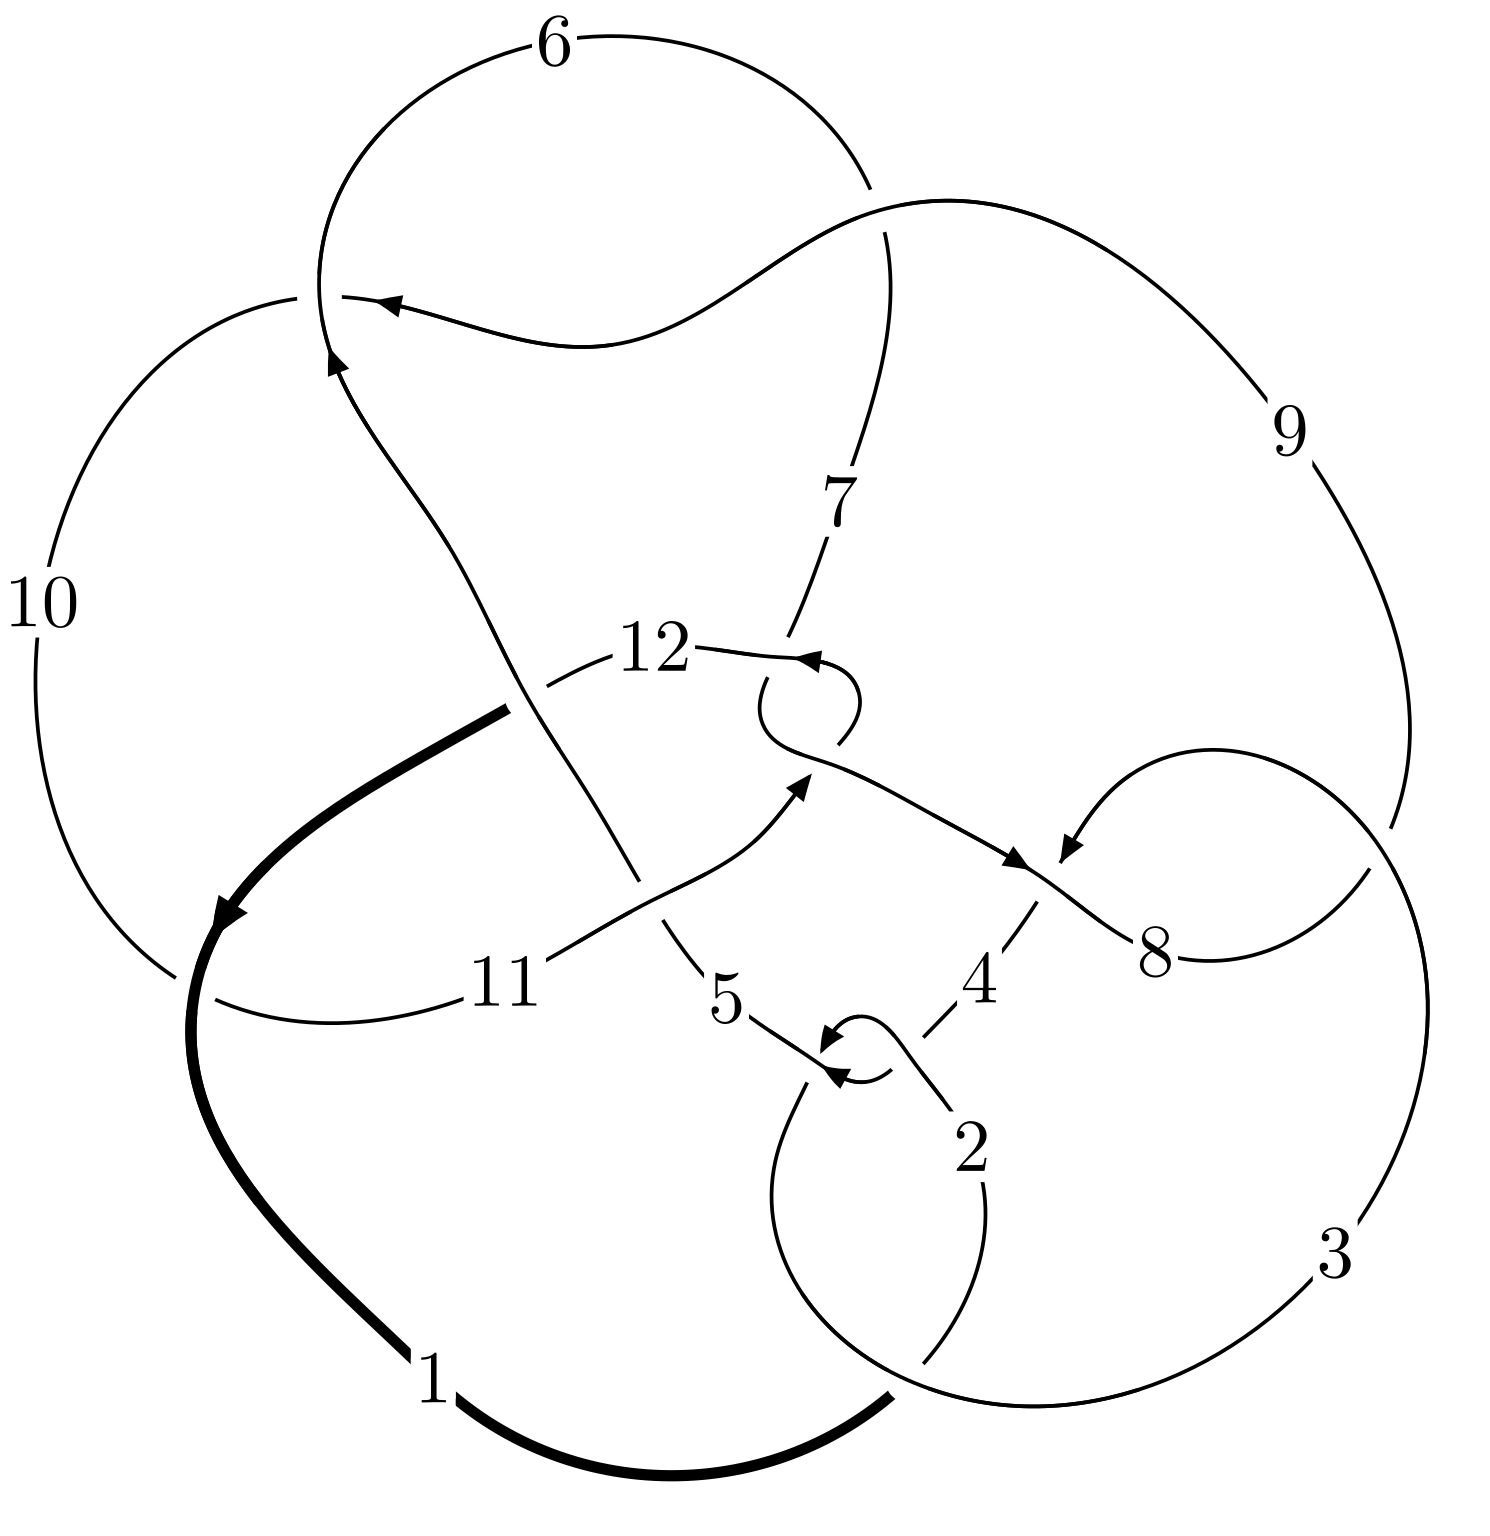
\includegraphics[width=112pt]{../../../GIT/diagram.site/Diagrams/png/2343_12n_0254.png}\\
\ \ \ A knot diagram\footnotemark}&
\allowdisplaybreaks
\textbf{Linearized knot diagam} \\
\cline{2-2}
 &
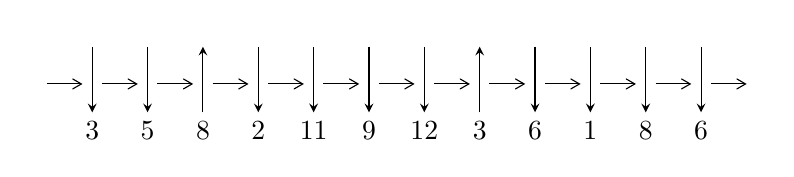
\begin{tikzpicture}[x=20pt, y=17pt]
	% nodes
	\node (C0) at (0, 0) {};
	\node (C1) at (1, 0) {};
	\node (C1U) at (1, +1) {};
	\node (C1D) at (1, -1) {3};

	\node (C2) at (2, 0) {};
	\node (C2U) at (2, +1) {};
	\node (C2D) at (2, -1) {5};

	\node (C3) at (3, 0) {};
	\node (C3U) at (3, +1) {};
	\node (C3D) at (3, -1) {8};

	\node (C4) at (4, 0) {};
	\node (C4U) at (4, +1) {};
	\node (C4D) at (4, -1) {2};

	\node (C5) at (5, 0) {};
	\node (C5U) at (5, +1) {};
	\node (C5D) at (5, -1) {11};

	\node (C6) at (6, 0) {};
	\node (C6U) at (6, +1) {};
	\node (C6D) at (6, -1) {9};

	\node (C7) at (7, 0) {};
	\node (C7U) at (7, +1) {};
	\node (C7D) at (7, -1) {12};

	\node (C8) at (8, 0) {};
	\node (C8U) at (8, +1) {};
	\node (C8D) at (8, -1) {3};

	\node (C9) at (9, 0) {};
	\node (C9U) at (9, +1) {};
	\node (C9D) at (9, -1) {6};

	\node (C10) at (10, 0) {};
	\node (C10U) at (10, +1) {};
	\node (C10D) at (10, -1) {1};

	\node (C11) at (11, 0) {};
	\node (C11U) at (11, +1) {};
	\node (C11D) at (11, -1) {8};

	\node (C12) at (12, 0) {};
	\node (C12U) at (12, +1) {};
	\node (C12D) at (12, -1) {6};
	\node (C13) at (13, 0) {};

	% arrows
	\draw[->,>={angle 60}]
	(C0) edge (C1) (C1) edge (C2) (C2) edge (C3) (C3) edge (C4) (C4) edge (C5) (C5) edge (C6) (C6) edge (C7) (C7) edge (C8) (C8) edge (C9) (C9) edge (C10) (C10) edge (C11) (C11) edge (C12) (C12) edge (C13) ;	\draw[->,>=stealth]
	(C1U) edge (C1D) (C2U) edge (C2D) (C3D) edge (C3U) (C4U) edge (C4D) (C5U) edge (C5D) (C6U) edge (C6D) (C7U) edge (C7D) (C8D) edge (C8U) (C9U) edge (C9D) (C10U) edge (C10D) (C11U) edge (C11D) (C12U) edge (C12D) ;
	\end{tikzpicture} \\
\hhline{~~} \\& 
\textbf{Solving Sequence} \\ \cline{2-2} 
 &
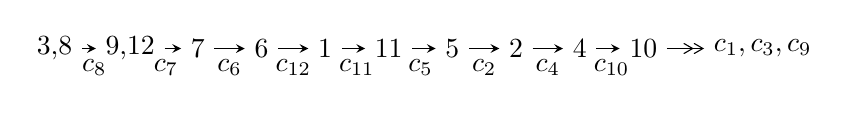
\begin{tikzpicture}[x=23pt, y=7pt]
	% node
	\node (A0) at (-1/8, 0) {3,8};
	\node (A1) at (17/16, 0) {9,12};
	\node (A2) at (17/8, 0) {7};
	\node (A3) at (25/8, 0) {6};
	\node (A4) at (33/8, 0) {1};
	\node (A5) at (41/8, 0) {11};
	\node (A6) at (49/8, 0) {5};
	\node (A7) at (57/8, 0) {2};
	\node (A8) at (65/8, 0) {4};
	\node (A9) at (73/8, 0) {10};
	\node (C1) at (1/2, -1) {$c_{8}$};
	\node (C2) at (13/8, -1) {$c_{7}$};
	\node (C3) at (21/8, -1) {$c_{6}$};
	\node (C4) at (29/8, -1) {$c_{12}$};
	\node (C5) at (37/8, -1) {$c_{11}$};
	\node (C6) at (45/8, -1) {$c_{5}$};
	\node (C7) at (53/8, -1) {$c_{2}$};
	\node (C8) at (61/8, -1) {$c_{4}$};
	\node (C9) at (69/8, -1) {$c_{10}$};
	\node (A10) at (11, 0) {$c_{1},c_{3},c_{9}$};

	% edge
	\draw[->,>=stealth]	
	(A0) edge (A1) (A1) edge (A2) (A2) edge (A3) (A3) edge (A4) (A4) edge (A5) (A5) edge (A6) (A6) edge (A7) (A7) edge (A8) (A8) edge (A9) ;
	\draw[->>,>={angle 60}]	
	(A9) edge (A10);
\end{tikzpicture} \\ 

\end{tabular} \\

\footnotetext{
The image of knot diagram is generated by the software ``\textbf{Draw programme}" developed by Andrew Bartholomew(\url{http://www.layer8.co.uk/maths/draw/index.htm\#Running-draw}), where we modified some parts for our purpose(\url{https://github.com/CATsTAILs/LinksPainter}).
}\phantom \\ \newline 
\centering \textbf{Ideals for irreducible components\footnotemark of $X_{\text{par}}$} 
 
\begin{align*}
I^u_{1}&=\langle 
2.85386\times10^{22} u^{20}-1.50646\times10^{23} u^{19}+\cdots+1.12972\times10^{24} b+1.18141\times10^{25},\\
\phantom{I^u_{1}}&\phantom{= \langle  }4.93819\times10^{24} u^{20}-2.24476\times10^{25} u^{19}+\cdots+2.48538\times10^{25} a+6.80715\times10^{26},\\
\phantom{I^u_{1}}&\phantom{= \langle  }u^{21}-5 u^{20}+\cdots+528 u-64\rangle \\
I^u_{2}&=\langle 
-271 u^5 a^3-2553 u^5 a^2+\cdots+3664 a-2027,\;-2 u^5 a^3+u^5 a^2+\cdots-4 a-2,\;u^6+u^5- u^4-2 u^3+u+1\rangle \\
I^u_{3}&=\langle 
-17 u^{10}+21 u^9+46 u^8+6 u^7-188 u^6-125 u^5+284 u^4+136 u^3+86 u^2+356 b-512 u+71,\\
\phantom{I^u_{3}}&\phantom{= \langle  }-617 u^{10}+202 u^9+\cdots+178 a-1470,\;u^{11}-3 u^9+2 u^7+5 u^6+u^5-4 u^4+6 u^3-2 u^2+u+1\rangle \\
\\
I^v_{1}&=\langle 
a,\;b+2 v+2,\;4 v^2+6 v+1\rangle \\
\end{align*}
\raggedright * 4 irreducible components of $\dim_{\mathbb{C}}=0$, with total 58 representations.\\
\footnotetext{All coefficients of polynomials are rational numbers. But the coefficients are sometimes approximated in decimal forms when there is not enough margin.}
\newpage
\renewcommand{\arraystretch}{1}
\centering \section*{I. $I^u_{1}= \langle 2.85\times10^{22} u^{20}-1.51\times10^{23} u^{19}+\cdots+1.13\times10^{24} b+1.18\times10^{25},\;4.94\times10^{24} u^{20}-2.24\times10^{25} u^{19}+\cdots+2.49\times10^{25} a+6.81\times10^{26},\;u^{21}-5 u^{20}+\cdots+528 u-64 \rangle$}
\flushleft \textbf{(i) Arc colorings}\\
\begin{tabular}{m{7pt} m{180pt} m{7pt} m{180pt} }
\flushright $a_{3}=$&$\begin{pmatrix}0\\u\end{pmatrix}$ \\
\flushright $a_{8}=$&$\begin{pmatrix}1\\0\end{pmatrix}$ \\
\flushright $a_{9}=$&$\begin{pmatrix}1\\- u^2\end{pmatrix}$ \\
\flushright $a_{12}=$&$\begin{pmatrix}-0.198690 u^{20}+0.903187 u^{19}+\cdots+168.839 u-27.3888\\-0.0252617 u^{20}+0.133349 u^{19}+\cdots+44.8453 u-10.4576\end{pmatrix}$ \\
\flushright $a_{7}=$&$\begin{pmatrix}-0.0389223 u^{20}+0.169523 u^{19}+\cdots+22.6922 u-1.25931\\-0.204843 u^{20}+0.945787 u^{19}+\cdots+195.515 u-36.3690\end{pmatrix}$ \\
\flushright $a_{6}=$&$\begin{pmatrix}-0.256774 u^{20}+1.17458 u^{19}+\cdots+228.962 u-39.2339\\-0.169105 u^{20}+0.785773 u^{19}+\cdots+165.000 u-30.9802\end{pmatrix}$ \\
\flushright $a_{1}=$&$\begin{pmatrix}-0.126591 u^{20}+0.558334 u^{19}+\cdots+86.6544 u-10.5130\\0.416280 u^{20}-1.91677 u^{19}+\cdots-391.813 u+72.1250\end{pmatrix}$ \\
\flushright $a_{11}=$&$\begin{pmatrix}-0.223951 u^{20}+1.03654 u^{19}+\cdots+213.684 u-37.8464\\-0.0252617 u^{20}+0.133349 u^{19}+\cdots+44.8453 u-10.4576\end{pmatrix}$ \\
\flushright $a_{5}=$&$\begin{pmatrix}-0.500539 u^{20}+2.28989 u^{19}+\cdots+447.169 u-77.8622\\-0.373948 u^{20}+1.73156 u^{19}+\cdots+360.515 u-67.3492\end{pmatrix}$ \\
\flushright $a_{2}=$&$\begin{pmatrix}-0.126591 u^{20}+0.558334 u^{19}+\cdots+86.6544 u-10.5130\\0.373948 u^{20}-1.73156 u^{19}+\cdots-360.515 u+67.3492\end{pmatrix}$ \\
\flushright $a_{4}=$&$\begin{pmatrix}- u\\- u\end{pmatrix}$ \\
\flushright $a_{10}=$&$\begin{pmatrix}0.0720983 u^{20}-0.344853 u^{19}+\cdots-82.1841 u+17.8758\\0.441542 u^{20}-2.05012 u^{19}+\cdots-436.659 u+82.5826\end{pmatrix}$\\&\end{tabular}
\flushleft \textbf{(ii) Obstruction class $= -1$}\\~\\
\flushleft \textbf{(iii) Cusp Shapes $= \frac{59011690898372144363232697}{49707567109353239097754688} u^{20}-\frac{278177987921238114159260841}{49707567109353239097754688} u^{19}+\cdots-\frac{15717053070456132195264300185}{12426891777338309774438672} u+\frac{380289254330637407319519649}{1553361472167288721804834}$}\\~\\
\newpage\renewcommand{\arraystretch}{1}
\flushleft \textbf{(iv) u-Polynomials at the component}\newline \\
\begin{tabular}{m{50pt}|m{274pt}}
Crossings & \hspace{64pt}u-Polynomials at each crossing \\
\hline $$\begin{aligned}c_{1}\end{aligned}$$&$\begin{aligned}
&u^{21}+11 u^{20}+\cdots+2416 u+256
\end{aligned}$\\
\hline $$\begin{aligned}c_{2},c_{4}\end{aligned}$$&$\begin{aligned}
&u^{21}-3 u^{20}+\cdots-12 u+16
\end{aligned}$\\
\hline $$\begin{aligned}c_{3},c_{8}\end{aligned}$$&$\begin{aligned}
&u^{21}+5 u^{20}+\cdots+528 u+64
\end{aligned}$\\
\hline $$\begin{aligned}c_{5},c_{7},c_{11}\end{aligned}$$&$\begin{aligned}
&u^{21}- u^{20}+\cdots-2 u+1
\end{aligned}$\\
\hline $$\begin{aligned}c_{6},c_{9},c_{12}\end{aligned}$$&$\begin{aligned}
&u^{21}-15 u^{19}+\cdots+3 u-1
\end{aligned}$\\
\hline $$\begin{aligned}c_{10}\end{aligned}$$&$\begin{aligned}
&u^{21}-19 u^{20}+\cdots+96 u-64
\end{aligned}$\\
\hline
\end{tabular}\\~\\
\newpage\renewcommand{\arraystretch}{1}
\flushleft \textbf{(v) Riley Polynomials at the component}\newline \\
\begin{tabular}{m{50pt}|m{274pt}}
Crossings & \hspace{64pt}Riley Polynomials at each crossing \\
\hline $$\begin{aligned}c_{1}\end{aligned}$$&$\begin{aligned}
&y^{21}+y^{20}+\cdots-37120 y-65536
\end{aligned}$\\
\hline $$\begin{aligned}c_{2},c_{4}\end{aligned}$$&$\begin{aligned}
&y^{21}-11 y^{20}+\cdots+2416 y-256
\end{aligned}$\\
\hline $$\begin{aligned}c_{3},c_{8}\end{aligned}$$&$\begin{aligned}
&y^{21}-9 y^{20}+\cdots+54016 y-4096
\end{aligned}$\\
\hline $$\begin{aligned}c_{5},c_{7},c_{11}\end{aligned}$$&$\begin{aligned}
&y^{21}+13 y^{20}+\cdots+46 y^2-1
\end{aligned}$\\
\hline $$\begin{aligned}c_{6},c_{9},c_{12}\end{aligned}$$&$\begin{aligned}
&y^{21}-30 y^{20}+\cdots+41 y-1
\end{aligned}$\\
\hline $$\begin{aligned}c_{10}\end{aligned}$$&$\begin{aligned}
&y^{21}-11 y^{20}+\cdots+115712 y-4096
\end{aligned}$\\
\hline
\end{tabular}\\~\\
\newpage\flushleft \textbf{(vi) Complex Volumes and Cusp Shapes}
$$\begin{array}{c|c|c}  
\text{Solutions to }I^u_{1}& \I (\text{vol} + \sqrt{-1}CS) & \text{Cusp shape}\\
 \hline 
\begin{aligned}
u &= -0.121943 + 0.682474 I \\
a &= \phantom{-}0.563394 - 0.200224 I \\
b &= \phantom{-}0.242967 + 0.329112 I\end{aligned}
 & -0.472540 - 0.941822 I & -7.59562 + 7.26185 I \\ \hline\begin{aligned}
u &= -0.121943 - 0.682474 I \\
a &= \phantom{-}0.563394 + 0.200224 I \\
b &= \phantom{-}0.242967 - 0.329112 I\end{aligned}
 & -0.472540 + 0.941822 I & -7.59562 - 7.26185 I \\ \hline\begin{aligned}
u &= \phantom{-}0.603944\phantom{ +0.000000I} \\
a &= \phantom{-}0.453168\phantom{ +0.000000I} \\
b &= \phantom{-}0.799712\phantom{ +0.000000I}\end{aligned}
 & -1.50093\phantom{ +0.000000I} & -5.01190\phantom{ +0.000000I} \\ \hline\begin{aligned}
u &= \phantom{-}0.536882 + 1.288830 I \\
a &= \phantom{-}0.332371 + 0.204687 I \\
b &= -0.203835 - 0.523003 I\end{aligned}
 & -7.32268 + 3.73921 I & -2.18512 - 2.93436 I \\ \hline\begin{aligned}
u &= \phantom{-}0.536882 - 1.288830 I \\
a &= \phantom{-}0.332371 - 0.204687 I \\
b &= -0.203835 + 0.523003 I\end{aligned}
 & -7.32268 - 3.73921 I & -2.18512 + 2.93436 I \\ \hline\begin{aligned}
u &= -0.45031 + 1.42697 I \\
a &= \phantom{-}0.401321 - 0.196262 I \\
b &= -0.169622 + 1.002850 I\end{aligned}
 & -0.856656 + 0.283512 I & -6.72739 - 0.35031 I \\ \hline\begin{aligned}
u &= -0.45031 - 1.42697 I \\
a &= \phantom{-}0.401321 + 0.196262 I \\
b &= -0.169622 - 1.002850 I\end{aligned}
 & -0.856656 - 0.283512 I & -6.72739 + 0.35031 I \\ \hline\begin{aligned}
u &= \phantom{-}1.39749 + 0.58008 I \\
a &= \phantom{-}0.000890 + 1.116300 I \\
b &= \phantom{-}0.416233 - 1.089790 I\end{aligned}
 & -3.89482 + 3.14186 I & -8.38778 - 3.45220 I \\ \hline\begin{aligned}
u &= \phantom{-}1.39749 - 0.58008 I \\
a &= \phantom{-}0.000890 - 1.116300 I \\
b &= \phantom{-}0.416233 + 1.089790 I\end{aligned}
 & -3.89482 - 3.14186 I & -8.38778 + 3.45220 I \\ \hline\begin{aligned}
u &= \phantom{-}0.452501\phantom{ +0.000000I} \\
a &= \phantom{-}2.15908\phantom{ +0.000000I} \\
b &= -0.287661\phantom{ +0.000000I}\end{aligned}
 & -2.05646\phantom{ +0.000000I} & -0.974600\phantom{ +0.000000I}\\
 \hline 
 \end{array}$$\newpage$$\begin{array}{c|c|c}  
\text{Solutions to }I^u_{1}& \I (\text{vol} + \sqrt{-1}CS) & \text{Cusp shape}\\
 \hline 
\begin{aligned}
u &= \phantom{-}0.68409 + 1.39512 I \\
a &= \phantom{-}0.435024 + 0.190053 I \\
b &= -0.549126 - 1.238180 I\end{aligned}
 & -2.93350 - 6.63406 I & -8.79219 + 4.92171 I \\ \hline\begin{aligned}
u &= \phantom{-}0.68409 - 1.39512 I \\
a &= \phantom{-}0.435024 - 0.190053 I \\
b &= -0.549126 + 1.238180 I\end{aligned}
 & -2.93350 + 6.63406 I & -8.79219 - 4.92171 I \\ \hline\begin{aligned}
u &= \phantom{-}1.30096 + 0.91198 I \\
a &= \phantom{-}0.393242 + 1.276420 I \\
b &= \phantom{-}0.90620 - 1.50613 I\end{aligned}
 & -0.8291 + 14.7385 I & -8.45146 - 7.52643 I \\ \hline\begin{aligned}
u &= \phantom{-}1.30096 - 0.91198 I \\
a &= \phantom{-}0.393242 - 1.276420 I \\
b &= \phantom{-}0.90620 + 1.50613 I\end{aligned}
 & -0.8291 - 14.7385 I & -8.45146 + 7.52643 I \\ \hline\begin{aligned}
u &= -1.42639 + 0.82761 I \\
a &= \phantom{-}0.254534 - 1.154900 I \\
b &= \phantom{-}0.63940 + 1.47836 I\end{aligned}
 & \phantom{-}2.34232 - 8.31871 I & -5.94131 + 4.58592 I \\ \hline\begin{aligned}
u &= -1.42639 - 0.82761 I \\
a &= \phantom{-}0.254534 + 1.154900 I \\
b &= \phantom{-}0.63940 - 1.47836 I\end{aligned}
 & \phantom{-}2.34232 + 8.31871 I & -5.94131 - 4.58592 I \\ \hline\begin{aligned}
u &= \phantom{-}0.334496\phantom{ +0.000000I} \\
a &= \phantom{-}0.508543\phantom{ +0.000000I} \\
b &= -1.69359\phantom{ +0.000000I}\end{aligned}
 & -10.4004\phantom{ +0.000000I} & \phantom{-}21.7570\phantom{ +0.000000I} \\ \hline\begin{aligned}
u &= \phantom{-}1.62920 + 0.48052 I \\
a &= -0.319293 - 1.001180 I \\
b &= -0.737374 + 0.986244 I\end{aligned}
 & \phantom{-}5.91302 + 6.12351 I & -10.80009 - 6.57387 I \\ \hline\begin{aligned}
u &= \phantom{-}1.62920 - 0.48052 I \\
a &= -0.319293 + 1.001180 I \\
b &= -0.737374 - 0.986244 I\end{aligned}
 & \phantom{-}5.91302 - 6.12351 I & -10.80009 + 6.57387 I \\ \hline\begin{aligned}
u &= -1.74543 + 0.04421 I \\
a &= -0.121882 + 0.958359 I \\
b &= -0.454067 - 1.159470 I\end{aligned}
 & \phantom{-}6.80819 + 0.98118 I & -9.12937 - 0.92113 I\\
 \hline 
 \end{array}$$\newpage$$\begin{array}{c|c|c}  
\text{Solutions to }I^u_{1}& \I (\text{vol} + \sqrt{-1}CS) & \text{Cusp shape}\\
 \hline 
\begin{aligned}
u &= -1.74543 - 0.04421 I \\
a &= -0.121882 - 0.958359 I \\
b &= -0.454067 + 1.159470 I\end{aligned}
 & \phantom{-}6.80819 - 0.98118 I & -9.12937 + 0.92113 I\\
 \hline 
 \end{array}$$\newpage\newpage\renewcommand{\arraystretch}{1}
\centering \section*{II. $I^u_{2}= \langle -271 u^5 a^3-2553 u^5 a^2+\cdots+3664 a-2027,\;-2 u^5 a^3+u^5 a^2+\cdots-4 a-2,\;u^6+u^5- u^4-2 u^3+u+1 \rangle$}
\flushleft \textbf{(i) Arc colorings}\\
\begin{tabular}{m{7pt} m{180pt} m{7pt} m{180pt} }
\flushright $a_{3}=$&$\begin{pmatrix}0\\u\end{pmatrix}$ \\
\flushright $a_{8}=$&$\begin{pmatrix}1\\0\end{pmatrix}$ \\
\flushright $a_{9}=$&$\begin{pmatrix}1\\- u^2\end{pmatrix}$ \\
\flushright $a_{12}=$&$\begin{pmatrix}a\\0.110657 a^{3} u^{5}+1.04247 a^{2} u^{5}+\cdots-1.49612 a+0.827685\end{pmatrix}$ \\
\flushright $a_{7}=$&$\begin{pmatrix}0.518579 a^{3} u^{5}+0.461004 a^{2} u^{5}+\cdots+0.0661494 a+0.956309\\-1.96366 a^{3} u^{5}-0.801552 a^{2} u^{5}+\cdots-1.76072 a-1.99755\end{pmatrix}$ \\
\flushright $a_{6}=$&$\begin{pmatrix}-0.518579 a^{3} u^{5}-0.461004 a^{2} u^{5}+\cdots-0.0661494 a-0.956309\\-0.110657 a^{3} u^{5}-1.04247 a^{2} u^{5}+\cdots+1.49612 a+0.172315\end{pmatrix}$ \\
\flushright $a_{1}=$&$\begin{pmatrix}u^2-1\\u^2\end{pmatrix}$ \\
\flushright $a_{11}=$&$\begin{pmatrix}0.110657 a^{3} u^{5}+1.04247 a^{2} u^{5}+\cdots-0.496121 a+0.827685\\0.110657 a^{3} u^{5}+1.04247 a^{2} u^{5}+\cdots-1.49612 a+0.827685\end{pmatrix}$ \\
\flushright $a_{5}=$&$\begin{pmatrix}- u^4+u^2-1\\- u^4\end{pmatrix}$ \\
\flushright $a_{2}=$&$\begin{pmatrix}u^2-1\\u^4\end{pmatrix}$ \\
\flushright $a_{4}=$&$\begin{pmatrix}- u\\- u\end{pmatrix}$ \\
\flushright $a_{10}=$&$\begin{pmatrix}-1.32993 a^{3} u^{5}+1.68150 a^{2} u^{5}+\cdots-2.77909 a+0.292364\\-1.44059 a^{3} u^{5}+0.639036 a^{2} u^{5}+\cdots-2.28297 a-0.535321\end{pmatrix}$\\&\end{tabular}
\flushleft \textbf{(ii) Obstruction class $= -1$}\\~\\
\flushleft \textbf{(iii) Cusp Shapes $= -4 u^4+4 u^2+4 u-10$}\\~\\
\newpage\renewcommand{\arraystretch}{1}
\flushleft \textbf{(iv) u-Polynomials at the component}\newline \\
\begin{tabular}{m{50pt}|m{274pt}}
Crossings & \hspace{64pt}u-Polynomials at each crossing \\
\hline $$\begin{aligned}c_{1}\end{aligned}$$&$\begin{aligned}
&(u^6+3 u^5+5 u^4+4 u^3+2 u^2+u+1)^4
\end{aligned}$\\
\hline $$\begin{aligned}c_{2},c_{3},c_{4}\\c_{8}\end{aligned}$$&$\begin{aligned}
&(u^6- u^5- u^4+2 u^3- u+1)^4
\end{aligned}$\\
\hline $$\begin{aligned}c_{5},c_{7},c_{11}\end{aligned}$$&$\begin{aligned}
&u^{24}+3 u^{23}+\cdots+418 u+319
\end{aligned}$\\
\hline $$\begin{aligned}c_{6},c_{9},c_{12}\end{aligned}$$&$\begin{aligned}
&u^{24}-3 u^{23}+\cdots-38 u+181
\end{aligned}$\\
\hline $$\begin{aligned}c_{10}\end{aligned}$$&$\begin{aligned}
&(u^2+u-1)^{12}
\end{aligned}$\\
\hline
\end{tabular}\\~\\
\newpage\renewcommand{\arraystretch}{1}
\flushleft \textbf{(v) Riley Polynomials at the component}\newline \\
\begin{tabular}{m{50pt}|m{274pt}}
Crossings & \hspace{64pt}Riley Polynomials at each crossing \\
\hline $$\begin{aligned}c_{1}\end{aligned}$$&$\begin{aligned}
&(y^6+y^5+5 y^4+6 y^2+3 y+1)^4
\end{aligned}$\\
\hline $$\begin{aligned}c_{2},c_{3},c_{4}\\c_{8}\end{aligned}$$&$\begin{aligned}
&(y^6-3 y^5+5 y^4-4 y^3+2 y^2- y+1)^4
\end{aligned}$\\
\hline $$\begin{aligned}c_{5},c_{7},c_{11}\end{aligned}$$&$\begin{aligned}
&y^{24}+11 y^{23}+\cdots+621500 y+101761
\end{aligned}$\\
\hline $$\begin{aligned}c_{6},c_{9},c_{12}\end{aligned}$$&$\begin{aligned}
&y^{24}-13 y^{23}+\cdots-152760 y+32761
\end{aligned}$\\
\hline $$\begin{aligned}c_{10}\end{aligned}$$&$\begin{aligned}
&(y^2-3 y+1)^{12}
\end{aligned}$\\
\hline
\end{tabular}\\~\\
\newpage\flushleft \textbf{(vi) Complex Volumes and Cusp Shapes}
$$\begin{array}{c|c|c}  
\text{Solutions to }I^u_{2}& \I (\text{vol} + \sqrt{-1}CS) & \text{Cusp shape}\\
 \hline 
\begin{aligned}
u &= \phantom{-}1.002190 + 0.295542 I \\
a &= -0.642556 - 0.992563 I \\
b &= -0.61676 + 1.29086 I\end{aligned}
 & \phantom{-}5.83845 + 0.92430 I & -4.28328 - 0.79423 I \\ \hline\begin{aligned}
u &= \phantom{-}1.002190 + 0.295542 I \\
a &= \phantom{-}0.85932 - 1.36236 I \\
b &= \phantom{-}0.022966 + 0.740302 I\end{aligned}
 & -2.05724 + 0.92430 I & -4.28328 - 0.79423 I \\ \hline\begin{aligned}
u &= \phantom{-}1.002190 + 0.295542 I \\
a &= \phantom{-}0.30955 + 1.60690 I \\
b &= \phantom{-}0.04999 - 1.65697 I\end{aligned}
 & \phantom{-}5.83845 + 0.92430 I & -4.28328 - 0.79423 I \\ \hline\begin{aligned}
u &= \phantom{-}1.002190 + 0.295542 I \\
a &= \phantom{-}0.012501 - 0.246000 I \\
b &= \phantom{-}1.46084 + 0.21819 I\end{aligned}
 & -2.05724 + 0.92430 I & -4.28328 - 0.79423 I \\ \hline\begin{aligned}
u &= \phantom{-}1.002190 - 0.295542 I \\
a &= -0.642556 + 0.992563 I \\
b &= -0.61676 - 1.29086 I\end{aligned}
 & \phantom{-}5.83845 - 0.92430 I & -4.28328 + 0.79423 I \\ \hline\begin{aligned}
u &= \phantom{-}1.002190 - 0.295542 I \\
a &= \phantom{-}0.85932 + 1.36236 I \\
b &= \phantom{-}0.022966 - 0.740302 I\end{aligned}
 & -2.05724 - 0.92430 I & -4.28328 + 0.79423 I \\ \hline\begin{aligned}
u &= \phantom{-}1.002190 - 0.295542 I \\
a &= \phantom{-}0.30955 - 1.60690 I \\
b &= \phantom{-}0.04999 + 1.65697 I\end{aligned}
 & \phantom{-}5.83845 - 0.92430 I & -4.28328 + 0.79423 I \\ \hline\begin{aligned}
u &= \phantom{-}1.002190 - 0.295542 I \\
a &= \phantom{-}0.012501 + 0.246000 I \\
b &= \phantom{-}1.46084 - 0.21819 I\end{aligned}
 & -2.05724 - 0.92430 I & -4.28328 + 0.79423 I \\ \hline\begin{aligned}
u &= -0.428243 + 0.664531 I \\
a &= -1.40914 + 1.08956 I \\
b &= \phantom{-}0.634044 - 0.520697 I\end{aligned}
 & -5.83845 + 0.92430 I & -11.71672 - 0.79423 I \\ \hline\begin{aligned}
u &= -0.428243 + 0.664531 I \\
a &= -0.93092 - 1.84591 I \\
b &= \phantom{-}0.192218 - 1.006480 I\end{aligned}
 & \phantom{-}2.05724 + 0.92430 I & -11.71672 - 0.79423 I\\
 \hline 
 \end{array}$$\newpage$$\begin{array}{c|c|c}  
\text{Solutions to }I^u_{2}& \I (\text{vol} + \sqrt{-1}CS) & \text{Cusp shape}\\
 \hline 
\begin{aligned}
u &= -0.428243 + 0.664531 I \\
a &= \phantom{-}2.36603 + 0.04486 I \\
b &= -0.032636 + 1.358240 I\end{aligned}
 & \phantom{-}2.05724 + 0.92430 I & -11.71672 - 0.79423 I \\ \hline\begin{aligned}
u &= -0.428243 + 0.664531 I \\
a &= -2.34802 + 3.62566 I \\
b &= -1.051840 - 0.400227 I\end{aligned}
 & -5.83845 + 0.92430 I & -11.71672 - 0.79423 I \\ \hline\begin{aligned}
u &= -0.428243 - 0.664531 I \\
a &= -1.40914 - 1.08956 I \\
b &= \phantom{-}0.634044 + 0.520697 I\end{aligned}
 & -5.83845 - 0.92430 I & -11.71672 + 0.79423 I \\ \hline\begin{aligned}
u &= -0.428243 - 0.664531 I \\
a &= -0.93092 + 1.84591 I \\
b &= \phantom{-}0.192218 + 1.006480 I\end{aligned}
 & \phantom{-}2.05724 - 0.92430 I & -11.71672 + 0.79423 I \\ \hline\begin{aligned}
u &= -0.428243 - 0.664531 I \\
a &= \phantom{-}2.36603 - 0.04486 I \\
b &= -0.032636 - 1.358240 I\end{aligned}
 & \phantom{-}2.05724 - 0.92430 I & -11.71672 + 0.79423 I \\ \hline\begin{aligned}
u &= -0.428243 - 0.664531 I \\
a &= -2.34802 - 3.62566 I \\
b &= -1.051840 + 0.400227 I\end{aligned}
 & -5.83845 - 0.92430 I & -11.71672 + 0.79423 I \\ \hline\begin{aligned}
u &= -1.073950 + 0.558752 I \\
a &= \phantom{-}0.461962 - 1.241720 I \\
b &= \phantom{-}0.48362 + 1.59891 I\end{aligned}
 & \phantom{-}3.94784 - 5.69302 I & -8.00000 + 5.51057 I \\ \hline\begin{aligned}
u &= -1.073950 + 0.558752 I \\
a &= -0.327999 + 0.551063 I \\
b &= -1.003490 - 0.857180 I\end{aligned}
 & \phantom{-}3.94784 - 5.69302 I & -8.00000 + 5.51057 I \\ \hline\begin{aligned}
u &= -1.073950 + 0.558752 I \\
a &= -0.370228 + 0.210083 I \\
b &= \phantom{-}1.67733 - 0.62104 I\end{aligned}
 & -3.94784 - 5.69302 I & -8.00000 + 5.51057 I \\ \hline\begin{aligned}
u &= -1.073950 + 0.558752 I \\
a &= \phantom{-}0.01951 + 1.59808 I \\
b &= -0.316295 - 1.320830 I\end{aligned}
 & -3.94784 - 5.69302 I & -8.00000 + 5.51057 I\\
 \hline 
 \end{array}$$\newpage$$\begin{array}{c|c|c}  
\text{Solutions to }I^u_{2}& \I (\text{vol} + \sqrt{-1}CS) & \text{Cusp shape}\\
 \hline 
\begin{aligned}
u &= -1.073950 - 0.558752 I \\
a &= \phantom{-}0.461962 + 1.241720 I \\
b &= \phantom{-}0.48362 - 1.59891 I\end{aligned}
 & \phantom{-}3.94784 + 5.69302 I & -8.00000 - 5.51057 I \\ \hline\begin{aligned}
u &= -1.073950 - 0.558752 I \\
a &= -0.327999 - 0.551063 I \\
b &= -1.003490 + 0.857180 I\end{aligned}
 & \phantom{-}3.94784 + 5.69302 I & -8.00000 - 5.51057 I \\ \hline\begin{aligned}
u &= -1.073950 - 0.558752 I \\
a &= -0.370228 - 0.210083 I \\
b &= \phantom{-}1.67733 + 0.62104 I\end{aligned}
 & -3.94784 + 5.69302 I & -8.00000 - 5.51057 I \\ \hline\begin{aligned}
u &= -1.073950 - 0.558752 I \\
a &= \phantom{-}0.01951 - 1.59808 I \\
b &= -0.316295 + 1.320830 I\end{aligned}
 & -3.94784 + 5.69302 I & -8.00000 - 5.51057 I\\
 \hline 
 \end{array}$$\newpage\newpage\renewcommand{\arraystretch}{1}
\centering \section*{III. $I^u_{3}= \langle -17 u^{10}+21 u^9+\cdots+356 b+71,\;-617 u^{10}+202 u^9+\cdots+178 a-1470,\;u^{11}-3 u^9+\cdots+u+1 \rangle$}
\flushleft \textbf{(i) Arc colorings}\\
\begin{tabular}{m{7pt} m{180pt} m{7pt} m{180pt} }
\flushright $a_{3}=$&$\begin{pmatrix}0\\u\end{pmatrix}$ \\
\flushright $a_{8}=$&$\begin{pmatrix}1\\0\end{pmatrix}$ \\
\flushright $a_{9}=$&$\begin{pmatrix}1\\- u^2\end{pmatrix}$ \\
\flushright $a_{12}=$&$\begin{pmatrix}3.46629 u^{10}-1.13483 u^{9}+\cdots-13.9270 u+8.25843\\0.0477528 u^{10}-0.0589888 u^{9}+\cdots+1.43820 u-0.199438\end{pmatrix}$ \\
\flushright $a_{7}=$&$\begin{pmatrix}2.36798 u^{10}-0.278090 u^{9}+\cdots-9.50562 u+8.34551\\-0.00842697 u^{10}+0.216292 u^{9}+\cdots+0.893258 u+0.0646067\end{pmatrix}$ \\
\flushright $a_{6}=$&$\begin{pmatrix}2.99719 u^{10}-0.261236 u^{9}+\cdots-10.7022 u+8.68820\\-0.0758427 u^{10}+0.446629 u^{9}+\cdots+1.53933 u+0.0814607\end{pmatrix}$ \\
\flushright $a_{1}=$&$\begin{pmatrix}-0.705056 u^{10}+0.429775 u^{9}+\cdots+2.73596 u-1.26124\\-0.0365169 u^{10}+0.103933 u^{9}+\cdots+0.370787 u+0.446629\end{pmatrix}$ \\
\flushright $a_{11}=$&$\begin{pmatrix}3.51404 u^{10}-1.19382 u^{9}+\cdots-12.4888 u+8.05899\\0.0477528 u^{10}-0.0589888 u^{9}+\cdots+1.43820 u-0.199438\end{pmatrix}$ \\
\flushright $a_{5}=$&$\begin{pmatrix}0.637640 u^{10}-0.199438 u^{9}+\cdots-2.08989 u+1.27809\\-0.0674157 u^{10}+0.230337 u^{9}+\cdots+0.646067 u+0.0168539\end{pmatrix}$ \\
\flushright $a_{2}=$&$\begin{pmatrix}-0.705056 u^{10}+0.429775 u^{9}+\cdots+2.73596 u-1.26124\\-0.0674157 u^{10}+0.230337 u^{9}+\cdots+0.646067 u+0.0168539\end{pmatrix}$ \\
\flushright $a_{4}=$&$\begin{pmatrix}u\\u\end{pmatrix}$ \\
\flushright $a_{10}=$&$\begin{pmatrix}4.17135 u^{10}-1.56461 u^{9}+\cdots-16.6629 u+10.5197\\0.0842697 u^{10}-0.162921 u^{9}+\cdots+1.06742 u-0.646067\end{pmatrix}$\\&\end{tabular}
\flushleft \textbf{(ii) Obstruction class $= 1$}\\~\\
\flushleft \textbf{(iii) Cusp Shapes $= \frac{1809}{356} u^{10}-\frac{507}{356} u^9-\frac{2437}{178} u^8+\frac{665}{178} u^7+\frac{410}{89} u^6+\frac{8485}{356} u^5+\frac{653}{178} u^4-\frac{2875}{178} u^3+\frac{3149}{89} u^2-\frac{4741}{178} u+\frac{2863}{356}$}\\~\\
\newpage\renewcommand{\arraystretch}{1}
\flushleft \textbf{(iv) u-Polynomials at the component}\newline \\
\begin{tabular}{m{50pt}|m{274pt}}
Crossings & \hspace{64pt}u-Polynomials at each crossing \\
\hline $$\begin{aligned}c_{1}\end{aligned}$$&$\begin{aligned}
&u^{11}-6 u^{10}+\cdots-3 u-1
\end{aligned}$\\
\hline $$\begin{aligned}c_{2}\end{aligned}$$&$\begin{aligned}
&u^{11}+4 u^{10}+5 u^9-2 u^8-11 u^7-8 u^6+4 u^5+8 u^4+2 u^3-2 u^2- u-1
\end{aligned}$\\
\hline $$\begin{aligned}c_{3}\end{aligned}$$&$\begin{aligned}
&u^{11}-3 u^9+2 u^7-5 u^6+u^5+4 u^4+6 u^3+2 u^2+u-1
\end{aligned}$\\
\hline $$\begin{aligned}c_{4}\end{aligned}$$&$\begin{aligned}
&u^{11}-4 u^{10}+5 u^9+2 u^8-11 u^7+8 u^6+4 u^5-8 u^4+2 u^3+2 u^2- u+1
\end{aligned}$\\
\hline $$\begin{aligned}c_{5},c_{11}\end{aligned}$$&$\begin{aligned}
&u^{11}+3 u^9+3 u^8+3 u^7+6 u^6+3 u^5+2 u^4+2 u^3-2 u^2-3 u-1
\end{aligned}$\\
\hline $$\begin{aligned}c_{6},c_{12}\end{aligned}$$&$\begin{aligned}
&u^{11}-3 u^{10}+2 u^9+2 u^8-2 u^7+3 u^6-6 u^5+3 u^4-3 u^3+3 u^2+1
\end{aligned}$\\
\hline $$\begin{aligned}c_{7}\end{aligned}$$&$\begin{aligned}
&u^{11}+3 u^9-3 u^8+3 u^7-6 u^6+3 u^5-2 u^4+2 u^3+2 u^2-3 u+1
\end{aligned}$\\
\hline $$\begin{aligned}c_{8}\end{aligned}$$&$\begin{aligned}
&u^{11}-3 u^9+2 u^7+5 u^6+u^5-4 u^4+6 u^3-2 u^2+u+1
\end{aligned}$\\
\hline $$\begin{aligned}c_{9}\end{aligned}$$&$\begin{aligned}
&u^{11}+3 u^{10}+2 u^9-2 u^8-2 u^7-3 u^6-6 u^5-3 u^4-3 u^3-3 u^2-1
\end{aligned}$\\
\hline $$\begin{aligned}c_{10}\end{aligned}$$&$\begin{aligned}
&u^{11}-5 u^{10}+\cdots-3 u-9
\end{aligned}$\\
\hline
\end{tabular}\\~\\
\newpage\renewcommand{\arraystretch}{1}
\flushleft \textbf{(v) Riley Polynomials at the component}\newline \\
\begin{tabular}{m{50pt}|m{274pt}}
Crossings & \hspace{64pt}Riley Polynomials at each crossing \\
\hline $$\begin{aligned}c_{1}\end{aligned}$$&$\begin{aligned}
&y^{11}+2 y^{10}+\cdots+25 y-1
\end{aligned}$\\
\hline $$\begin{aligned}c_{2},c_{4}\end{aligned}$$&$\begin{aligned}
&y^{11}-6 y^{10}+\cdots-3 y-1
\end{aligned}$\\
\hline $$\begin{aligned}c_{3},c_{8}\end{aligned}$$&$\begin{aligned}
&y^{11}-6 y^{10}+\cdots+5 y-1
\end{aligned}$\\
\hline $$\begin{aligned}c_{5},c_{7},c_{11}\end{aligned}$$&$\begin{aligned}
&y^{11}+6 y^{10}+\cdots+5 y-1
\end{aligned}$\\
\hline $$\begin{aligned}c_{6},c_{9},c_{12}\end{aligned}$$&$\begin{aligned}
&y^{11}-5 y^{10}+\cdots-6 y-1
\end{aligned}$\\
\hline $$\begin{aligned}c_{10}\end{aligned}$$&$\begin{aligned}
&y^{11}-5 y^{10}+\cdots+369 y-81
\end{aligned}$\\
\hline
\end{tabular}\\~\\
\newpage\flushleft \textbf{(vi) Complex Volumes and Cusp Shapes}
$$\begin{array}{c|c|c}  
\text{Solutions to }I^u_{3}& \I (\text{vol} + \sqrt{-1}CS) & \text{Cusp shape}\\
 \hline 
\begin{aligned}
u &= \phantom{-}0.625397 + 0.494839 I \\
a &= \phantom{-}0.438748 - 1.244100 I \\
b &= \phantom{-}0.821829 + 0.139209 I\end{aligned}
 & -3.46083 + 0.46362 I & -10.64211 + 0.77158 I \\ \hline\begin{aligned}
u &= \phantom{-}0.625397 - 0.494839 I \\
a &= \phantom{-}0.438748 + 1.244100 I \\
b &= \phantom{-}0.821829 - 0.139209 I\end{aligned}
 & -3.46083 - 0.46362 I & -10.64211 - 0.77158 I \\ \hline\begin{aligned}
u &= -0.564447 + 1.125840 I \\
a &= -0.247928 + 0.345446 I \\
b &= \phantom{-}0.522992 - 0.276078 I\end{aligned}
 & -7.82119 - 3.76164 I & -18.6525 + 4.0849 I \\ \hline\begin{aligned}
u &= -0.564447 - 1.125840 I \\
a &= -0.247928 - 0.345446 I \\
b &= \phantom{-}0.522992 + 0.276078 I\end{aligned}
 & -7.82119 + 3.76164 I & -18.6525 - 4.0849 I \\ \hline\begin{aligned}
u &= \phantom{-}0.145041 + 0.670202 I \\
a &= \phantom{-}0.32779 + 2.44730 I \\
b &= \phantom{-}0.101556 + 1.234860 I\end{aligned}
 & \phantom{-}2.75970 - 0.49193 I & -4.46246 - 4.43880 I \\ \hline\begin{aligned}
u &= \phantom{-}0.145041 - 0.670202 I \\
a &= \phantom{-}0.32779 - 2.44730 I \\
b &= \phantom{-}0.101556 - 1.234860 I\end{aligned}
 & \phantom{-}2.75970 + 0.49193 I & -4.46246 + 4.43880 I \\ \hline\begin{aligned}
u &= -1.50834 + 0.06577 I \\
a &= -0.223191 + 1.141650 I \\
b &= -0.44883 - 1.38945 I\end{aligned}
 & \phantom{-}7.91909 + 0.79075 I & -1.37905 - 0.86737 I \\ \hline\begin{aligned}
u &= -1.50834 - 0.06577 I \\
a &= -0.223191 - 1.141650 I \\
b &= -0.44883 + 1.38945 I\end{aligned}
 & \phantom{-}7.91909 - 0.79075 I & -1.37905 + 0.86737 I \\ \hline\begin{aligned}
u &= \phantom{-}1.48572 + 0.56088 I \\
a &= -0.448099 - 0.943396 I \\
b &= -0.619533 + 1.131030 I\end{aligned}
 & \phantom{-}6.75307 + 5.68255 I & -2.50294 - 2.90690 I \\ \hline\begin{aligned}
u &= \phantom{-}1.48572 - 0.56088 I \\
a &= -0.448099 + 0.943396 I \\
b &= -0.619533 - 1.131030 I\end{aligned}
 & \phantom{-}6.75307 - 5.68255 I & -2.50294 + 2.90690 I\\
 \hline 
 \end{array}$$\newpage$$\begin{array}{c|c|c}  
\text{Solutions to }I^u_{3}& \I (\text{vol} + \sqrt{-1}CS) & \text{Cusp shape}\\
 \hline 
\begin{aligned}
u &= -0.366747\phantom{ +0.000000I} \\
a &= \phantom{-}17.3054\phantom{ +0.000000I} \\
b &= -0.756037\phantom{ +0.000000I}\end{aligned}
 & -5.71995\phantom{ +0.000000I} & \phantom{-}23.2780\phantom{ +0.000000I}\\
 \hline 
 \end{array}$$\newpage\newpage\renewcommand{\arraystretch}{1}
\centering \section*{IV. $I^v_{1}= \langle a,\;b+2 v+2,\;4 v^2+6 v+1 \rangle$}
\flushleft \textbf{(i) Arc colorings}\\
\begin{tabular}{m{7pt} m{180pt} m{7pt} m{180pt} }
\flushright $a_{3}=$&$\begin{pmatrix}v\\0\end{pmatrix}$ \\
\flushright $a_{8}=$&$\begin{pmatrix}1\\0\end{pmatrix}$ \\
\flushright $a_{9}=$&$\begin{pmatrix}1\\0\end{pmatrix}$ \\
\flushright $a_{12}=$&$\begin{pmatrix}0\\-2 v-2\end{pmatrix}$ \\
\flushright $a_{7}=$&$\begin{pmatrix}1\\-2 v-3\end{pmatrix}$ \\
\flushright $a_{6}=$&$\begin{pmatrix}-2 v-2\\-2 v-3\end{pmatrix}$ \\
\flushright $a_{1}=$&$\begin{pmatrix}4 v+5\\4 v+6\end{pmatrix}$ \\
\flushright $a_{11}=$&$\begin{pmatrix}-2 v-2\\-2 v-2\end{pmatrix}$ \\
\flushright $a_{5}=$&$\begin{pmatrix}-4 v-5\\-4 v-6\end{pmatrix}$ \\
\flushright $a_{2}=$&$\begin{pmatrix}5 v+5\\4 v+6\end{pmatrix}$ \\
\flushright $a_{4}=$&$\begin{pmatrix}v\\0\end{pmatrix}$ \\
\flushright $a_{10}=$&$\begin{pmatrix}4 v+6\\6 v+8\end{pmatrix}$\\&\end{tabular}
\flushleft \textbf{(ii) Obstruction class $= 1$}\\~\\
\flushleft \textbf{(iii) Cusp Shapes $= -\frac{45}{2} v-\frac{183}{4}$}\\~\\
\newpage\renewcommand{\arraystretch}{1}
\flushleft \textbf{(iv) u-Polynomials at the component}\newline \\
\begin{tabular}{m{50pt}|m{274pt}}
Crossings & \hspace{64pt}u-Polynomials at each crossing \\
\hline $$\begin{aligned}c_{1},c_{2}\end{aligned}$$&$\begin{aligned}
&(u-1)^2
\end{aligned}$\\
\hline $$\begin{aligned}c_{3},c_{8}\end{aligned}$$&$\begin{aligned}
&u^2
\end{aligned}$\\
\hline $$\begin{aligned}c_{4}\end{aligned}$$&$\begin{aligned}
&(u+1)^2
\end{aligned}$\\
\hline $$\begin{aligned}c_{5},c_{7},c_{10}\end{aligned}$$&$\begin{aligned}
&u^2+u-1
\end{aligned}$\\
\hline $$\begin{aligned}c_{6}\end{aligned}$$&$\begin{aligned}
&u^2-3 u+1
\end{aligned}$\\
\hline $$\begin{aligned}c_{9},c_{12}\end{aligned}$$&$\begin{aligned}
&u^2+3 u+1
\end{aligned}$\\
\hline $$\begin{aligned}c_{11}\end{aligned}$$&$\begin{aligned}
&u^2- u-1
\end{aligned}$\\
\hline
\end{tabular}\\~\\
\newpage\renewcommand{\arraystretch}{1}
\flushleft \textbf{(v) Riley Polynomials at the component}\newline \\
\begin{tabular}{m{50pt}|m{274pt}}
Crossings & \hspace{64pt}Riley Polynomials at each crossing \\
\hline $$\begin{aligned}c_{1},c_{2},c_{4}\end{aligned}$$&$\begin{aligned}
&(y-1)^2
\end{aligned}$\\
\hline $$\begin{aligned}c_{3},c_{8}\end{aligned}$$&$\begin{aligned}
&y^2
\end{aligned}$\\
\hline $$\begin{aligned}c_{5},c_{7},c_{10}\\c_{11}\end{aligned}$$&$\begin{aligned}
&y^2-3 y+1
\end{aligned}$\\
\hline $$\begin{aligned}c_{6},c_{9},c_{12}\end{aligned}$$&$\begin{aligned}
&y^2-7 y+1
\end{aligned}$\\
\hline
\end{tabular}\\~\\
\newpage\flushleft \textbf{(vi) Complex Volumes and Cusp Shapes}
$$\begin{array}{c|c|c}  
\text{Solutions to }I^v_{1}& \I (\text{vol} + \sqrt{-1}CS) & \text{Cusp shape}\\
 \hline 
\begin{aligned}
v &= -1.30902\phantom{ +0.000000I} \\
a &= \phantom{-0.000000 } 0 \\
b &= \phantom{-}0.618034\phantom{ +0.000000I}\end{aligned}
 & -2.63189\phantom{ +0.000000I} & -16.2970\phantom{ +0.000000I} \\ \hline\begin{aligned}
v &= -0.190983\phantom{ +0.000000I} \\
a &= \phantom{-0.000000 } 0 \\
b &= -1.61803\phantom{ +0.000000I}\end{aligned}
 & -10.5276\phantom{ +0.000000I} & -41.4530\phantom{ +0.000000I}\\
 \hline 
 \end{array}$$\newpage
\newpage\renewcommand{\arraystretch}{1}
\centering \section*{ V. u-Polynomials}
\begin{tabular}{m{50pt}|m{274pt}}
Crossings & \hspace{64pt}u-Polynomials at each crossing \\
\hline $$\begin{aligned}c_{1}\end{aligned}$$&$\begin{aligned}
&(u-1)^2(u^6+3 u^5+5 u^4+4 u^3+2 u^2+u+1)^4\\
&\cdot(u^{11}-6 u^{10}+\cdots-3 u-1)(u^{21}+11 u^{20}+\cdots+2416 u+256)
\end{aligned}$\\
\hline $$\begin{aligned}c_{2}\end{aligned}$$&$\begin{aligned}
&(u-1)^2(u^6- u^5- u^4+2 u^3- u+1)^4\\
&\cdot(u^{11}+4 u^{10}+5 u^9-2 u^8-11 u^7-8 u^6+4 u^5+8 u^4+2 u^3-2 u^2- u-1)\\
&\cdot(u^{21}-3 u^{20}+\cdots-12 u+16)
\end{aligned}$\\
\hline $$\begin{aligned}c_{3}\end{aligned}$$&$\begin{aligned}
&u^2(u^6- u^5- u^4+2 u^3- u+1)^4\\
&\cdot(u^{11}-3 u^9+2 u^7-5 u^6+u^5+4 u^4+6 u^3+2 u^2+u-1)\\
&\cdot(u^{21}+5 u^{20}+\cdots+528 u+64)
\end{aligned}$\\
\hline $$\begin{aligned}c_{4}\end{aligned}$$&$\begin{aligned}
&(u+1)^2(u^6- u^5- u^4+2 u^3- u+1)^4\\
&\cdot(u^{11}-4 u^{10}+5 u^9+2 u^8-11 u^7+8 u^6+4 u^5-8 u^4+2 u^3+2 u^2- u+1)\\
&\cdot(u^{21}-3 u^{20}+\cdots-12 u+16)
\end{aligned}$\\
\hline $$\begin{aligned}c_{5}\end{aligned}$$&$\begin{aligned}
&(u^2+u-1)\\
&\cdot(u^{11}+3 u^9+3 u^8+3 u^7+6 u^6+3 u^5+2 u^4+2 u^3-2 u^2-3 u-1)\\
&\cdot(u^{21}- u^{20}+\cdots-2 u+1)(u^{24}+3 u^{23}+\cdots+418 u+319)
\end{aligned}$\\
\hline $$\begin{aligned}c_{6}\end{aligned}$$&$\begin{aligned}
&(u^2-3 u+1)\\
&\cdot(u^{11}-3 u^{10}+2 u^9+2 u^8-2 u^7+3 u^6-6 u^5+3 u^4-3 u^3+3 u^2+1)\\
&\cdot(u^{21}-15 u^{19}+\cdots+3 u-1)(u^{24}-3 u^{23}+\cdots-38 u+181)
\end{aligned}$\\
\hline $$\begin{aligned}c_{7}\end{aligned}$$&$\begin{aligned}
&(u^2+u-1)\\
&\cdot(u^{11}+3 u^9-3 u^8+3 u^7-6 u^6+3 u^5-2 u^4+2 u^3+2 u^2-3 u+1)\\
&\cdot(u^{21}- u^{20}+\cdots-2 u+1)(u^{24}+3 u^{23}+\cdots+418 u+319)
\end{aligned}$\\
\hline $$\begin{aligned}c_{8}\end{aligned}$$&$\begin{aligned}
&u^2(u^6- u^5- u^4+2 u^3- u+1)^4\\
&\cdot(u^{11}-3 u^9+2 u^7+5 u^6+u^5-4 u^4+6 u^3-2 u^2+u+1)\\
&\cdot(u^{21}+5 u^{20}+\cdots+528 u+64)
\end{aligned}$\\
\hline $$\begin{aligned}c_{9}\end{aligned}$$&$\begin{aligned}
&(u^2+3 u+1)\\
&\cdot(u^{11}+3 u^{10}+2 u^9-2 u^8-2 u^7-3 u^6-6 u^5-3 u^4-3 u^3-3 u^2-1)\\
&\cdot(u^{21}-15 u^{19}+\cdots+3 u-1)(u^{24}-3 u^{23}+\cdots-38 u+181)
\end{aligned}$\\
\hline $$\begin{aligned}c_{10}\end{aligned}$$&$\begin{aligned}
&((u^2+u-1)^{13})(u^{11}-5 u^{10}+\cdots-3 u-9)(u^{21}-19 u^{20}+\cdots+96 u-64)
\end{aligned}$\\
\hline $$\begin{aligned}c_{11}\end{aligned}$$&$\begin{aligned}
&(u^2- u-1)\\
&\cdot(u^{11}+3 u^9+3 u^8+3 u^7+6 u^6+3 u^5+2 u^4+2 u^3-2 u^2-3 u-1)\\
&\cdot(u^{21}- u^{20}+\cdots-2 u+1)(u^{24}+3 u^{23}+\cdots+418 u+319)
\end{aligned}$\\
\hline $$\begin{aligned}c_{12}\end{aligned}$$&$\begin{aligned}
&(u^2+3 u+1)\\
&\cdot(u^{11}-3 u^{10}+2 u^9+2 u^8-2 u^7+3 u^6-6 u^5+3 u^4-3 u^3+3 u^2+1)\\
&\cdot(u^{21}-15 u^{19}+\cdots+3 u-1)(u^{24}-3 u^{23}+\cdots-38 u+181)
\end{aligned}$\\
\hline
\end{tabular}\newpage\renewcommand{\arraystretch}{1}
\centering \section*{ VI. Riley Polynomials}
\begin{tabular}{m{50pt}|m{274pt}}
Crossings & \hspace{64pt}Riley Polynomials at each crossing \\
\hline $$\begin{aligned}c_{1}\end{aligned}$$&$\begin{aligned}
&((y-1)^2)(y^6+y^5+\cdots+3 y+1)^{4}(y^{11}+2 y^{10}+\cdots+25 y-1)\\
&\cdot(y^{21}+y^{20}+\cdots-37120 y-65536)
\end{aligned}$\\
\hline $$\begin{aligned}c_{2},c_{4}\end{aligned}$$&$\begin{aligned}
&(y-1)^2(y^6-3 y^5+5 y^4-4 y^3+2 y^2- y+1)^4\\
&\cdot(y^{11}-6 y^{10}+\cdots-3 y-1)(y^{21}-11 y^{20}+\cdots+2416 y-256)
\end{aligned}$\\
\hline $$\begin{aligned}c_{3},c_{8}\end{aligned}$$&$\begin{aligned}
&y^2(y^6-3 y^5+\cdots- y+1)^{4}(y^{11}-6 y^{10}+\cdots+5 y-1)\\
&\cdot(y^{21}-9 y^{20}+\cdots+54016 y-4096)
\end{aligned}$\\
\hline $$\begin{aligned}c_{5},c_{7},c_{11}\end{aligned}$$&$\begin{aligned}
&(y^2-3 y+1)(y^{11}+6 y^{10}+\cdots+5 y-1)(y^{21}+13 y^{20}+\cdots+46 y^2-1)\\
&\cdot(y^{24}+11 y^{23}+\cdots+621500 y+101761)
\end{aligned}$\\
\hline $$\begin{aligned}c_{6},c_{9},c_{12}\end{aligned}$$&$\begin{aligned}
&(y^2-7 y+1)(y^{11}-5 y^{10}+\cdots-6 y-1)(y^{21}-30 y^{20}+\cdots+41 y-1)\\
&\cdot(y^{24}-13 y^{23}+\cdots-152760 y+32761)
\end{aligned}$\\
\hline $$\begin{aligned}c_{10}\end{aligned}$$&$\begin{aligned}
&((y^2-3 y+1)^{13})(y^{11}-5 y^{10}+\cdots+369 y-81)\\
&\cdot(y^{21}-11 y^{20}+\cdots+115712 y-4096)
\end{aligned}$\\
\hline
\end{tabular}
\vskip 2pc
\end{document}